\documentclass[5p,a4paper,english]{elsarticle}% 5p gir 2 kolonner pr side. 1p gir 1 kolonne pr side.
%\documentclass[11pt,a4paper,norsk]{article} % setter hvilken type dokument. Kan også være book eller report. I klammeparantes settes fontstørrelse, papirstørrelse og språk.

\usepackage[utf8]{inputenc} %- Løser problem med å skrive andre enn engelske bokstaver f.eks æ,ø,å.

\usepackage[T1]{fontenc} %- Støtter koding av forskjellige fonter.

\usepackage{textcomp} % Støtter bruk av forskjellige fonter som dollartegn, copyright, en kvart, en halv mm, se http://gcp.fcaglp.unlp.edu.ar/_media/integrantes:psantamaria:latex:textcomp.pdf

\usepackage{url} % Gjør internett- og e-mail adresser klikkbare i tex-dokumentet.

\usepackage{hyperref} % Gjør referansene i tex-dokumentet klikkbare, slik at du kommer til referansen i referanselista.

\usepackage[english]{babel} % Ordbok. Hvis man setter norsk i options til usepackage babel kan man bruke norske ord.

\usepackage{natbib}
\bibliographystyle{unsrtnat}

\urlstyle{sf} % Velger hvilken stil url-adresser skrives, f.eks sf

\usepackage{graphicx, subfig} % Brukes for å sette inn bilder eller figurer
\usepackage{amsmath} 				% Ekstra matematikkfunksjoner.
\usepackage{amssymb}
\usepackage{amsfonts}
\usepackage{amsthm}
\usepackage{mathrsfs}
\usepackage{mathtools}
\usepackage{geometry}
\usepackage{tikz-cd}
\usepackage{bm}
\usepackage{graphicx}
\usepackage{changepage}

\usepackage{siunitx}					% Må inkluderes for blant annet å få tilgang til kommandoen \SI (korrekte måltall med enheter)
	\sisetup{exponent-product = \cdot}      	% Prikk som multiplikasjonstegn (i steden for kryss).
 	\sisetup{output-decimal-marker  =  {,}} 	% Komma som desimalskilletegn (i steden for punktum).
 	\sisetup{separate-uncertainty = true}   	% Pluss-minus-form på usikkerhet (i steden for parentes). 

\usepackage{booktabs}                     		% For å få tilgang til finere linjer (til bruk i tabeller og slikt).

\usepackage[font=small,labelfont=bf]{caption}		% For justering av figurtekst og tabelltekst.

\journal{ }
\usepackage{etoolbox}
\makeatletter
\patchcmd{\ps@pprintTitle}
  {Preprint submitted to}
  {}
  {}{}
\makeatother
% Fjerner submitte dto 




% Denne setter navnet på abstract til Sammendrag
\renewenvironment{abstract}{\global\setbox\absbox=\vbox\bgroup
\hsize=\textwidth\def\baselinestretch{1}%
\noindent\unskip\textbf{Sammendrag}
\par\medskip\noindent\unskip\ignorespaces}
{\egroup}

%\clearpage % Bruk denne kommandoen dersom du vil ha ny side etter det er satt plass til figuren.
% Disse kommandoene kan gjøre det enklere for LaTeX å plassere figurer og tabeller der du ønsker.
\setcounter{totalnumber}{5}
\renewcommand{\textfraction}{0.05}
\renewcommand{\topfraction}{0.95}
\renewcommand{\bottomfraction}{0.95}
\renewcommand{\floatpagefraction}{0.35}


%%%%%%%%%%%%%%%%%%%%%%%%%%%%%%%%%%%%%%%%%%%%%%%%%%%%%%%%%%%%%%%%%%%%%%%%%
\begin{document}

\begin{frontmatter}

\title{Element method project 1}
\author[matematikk]{Håkon Noren}

\author[matematikk]{Alexander Johan Arntzen }

\address[matematikk]{Department of Mathematical Science, Norwegian University of Science and Technology, N-7491 Trondheim, Norway.}


\begin{abstract}
Lorem ipsum dolor sit amet, consectetur adipisicing elit, sed do eiusmod tempor incididunt ut labore et dolore magna aliqua. Ut enim ad minim veniam, quis nostrud exercitation ullamco laboris nisi ut aliquip ex ea commodo consequat. Duis aute irure dolor in reprehenderit in voluptate velit esse cillum dolore eu fugiat nulla pariatur. Excepteur sint occaecat cupidatat non proident, sunt in culpa qui officia deserunt mollit anim id est laborum.
\end{abstract}

\end{frontmatter}


%%%%%%%%%%%%%%%%%%%%%%%%%%%%%%%%%%%%%%%%%%%%%%%%%%%%%%%%%%%%%%%%%%%%%%%%%
\section{Innledning}
Lorem ipsum dolor sit amet, consectetur adipisicing elit, sed do eiusmod tempor incididunt ut labore et dolore magna aliqua. Ut enim ad minim veniam, quis nostrud exercitation ullamco laboris nisi ut aliquip ex ea commodo consequat. Duis aute irure dolor in reprehenderit in voluptate velit esse cillum dolore eu fugiat nulla pariatur. Excepteur sint occaecat cupidatat non proident, sunt in culpa qui officia deserunt mollit anim id est laborum.



%%%%%%%%%%%%%%%%%%%%%%%%%%%%%%%%%%%%%%%%%%%%%%%%%%%%%%%%%%%%%%%%%%%%%%%%%
\section{Teori}

\subsection{Problem}


Given the two dimensional Poisson problem

\begin{equation}
\begin{aligned}
    \nabla^2 u(x,y) &= - f(x,y)
    \\
    u(x,y) |_{r=1} &= 0
\label{poission-problem}
\end{aligned}
\end{equation}

on the domain $\Omega$ given by the unit disk

\begin{equation*}
    \Omega = \{(x,y) : x^2+ y^2 \leq 1 \}
\end{equation*}

with $f$ in polar coordinates given By

\begin{equation*}
f(r,\theta) = -8\pi\cos(2\pi r^2) + 16 \pi^2r^2 \sin(2\pi r^2)
\end{equation*}

\subsection{Analytical soluion}

Assume the following analytical solution

\begin{equation}
u(x,y) = \sin(2\pi (x^2 + y^2))
\end{equation}

which we easily verify with $g = g(x,y) = 2\pi (x^2 + y^2)$

\begin{equation*}
\begin{aligned}
\frac{\partial^2u}{\partial x^2} = u_{xx} &= 4\pi\cos(g) - 16\pi^2x^2\sin(g)
\\
u_{yy} &= 4\pi\cos(g) - 16\pi^2y^2\sin(g)
\end{aligned}
\end{equation*}

as $r^2 = x^2 + y^2$ we find 

\begin{equation*}
    \begin{aligned}
\nabla^2 u &= u_{xx} + u{yy}
\\
&= 8\pi \cos(2\pi r^2) - 16\pi^2r^2\sin(2\pi r^2)
\\
& = -f(x,y) & \qed
\end{aligned}
\end{equation*}





\subsection{Weak formulation}


The weak formulation is given by 


\begin{equation*}
\begin{aligned}
    a(u,v) &= \iint\limits_{\Omega} \nabla u \cdot \nabla v \, dx \, dy
    \\
    l(v) &= \iint\limits_{\Omega} fv \, dx \, dy
\end{aligned}
\end{equation*}

In our case we have

\begin{equation*}
\begin{aligned}
    \nabla^2u &=  -f
    \\
    \nabla^2uv &= -fv
    \\
     \iint\limits_{\Omega} \nabla^2uv \, dx \, dy &=  -\iint\limits_{\Omega} fv \, dx \, dy
    \\
    \end{aligned}
\end{equation*}

As $\nabla^2u = u_{xx} + u_{yy}$ we use integration by parts to find

\begin{equation*}
    \iint\limits_{\Omega} u_{xx}v \, dx \, dy 
    = \underbrace{u_xv |_{\partial \Omega}}_{=0} - \iint\limits_{\Omega} u_xv_x \, dx \, dy 
\end{equation*}
    

\begin{equation*}
\begin{aligned}
    \implies
    \iint\limits_{\Omega} \nabla^2uv \, dx \, dy &= \iint\limits_{\Omega} (u_xv_x + u_yv_y)v \, dx \, dy \\
    &= \iint\limits_{\Omega} \nabla u \cdot \nabla v \, dx \, dy 
\end{aligned}
\end{equation*}

Where we assumed that this holds  $\forall v \in X$ where we then have to assume that the space $X$ is defined By

\begin{equation*}
    \begin{aligned}
        X &= \{v \in H^1(\Omega) : v|_{\partial \Omega = 0} \} \\
         &= H^1_0(\Omega)
    \end{aligned}
\end{equation*}

\subsection{Galerkin projection}

We now search for solutions in the finite subspace $X_h \subset X$. 
By discretizing $\Omega$ into $M$ triangles $K_k$ defined by corner nodes $x_i$, we have basis functions corresponding to each node.
Let 

\begin{equation*}
X_h = \{ v \in X : v|_{K_k} \in \mathbb{P}_1 (K_k),1\leq k\leq M \}
\end{equation*}

and $\{\phi_i\}_{i=1}^n$ be the basis functions of $X_h$ such that

\begin{equation*}
    \begin{aligned}
X_h = \text{span} \{\phi_i\}_{i=1}^n & & \phi_j(x_i) = \delta_{ij}
    \end{aligned}
\end{equation*}

hence we aim to find $u_h \in X_h$ $\forall v \in X_h$, meaning we can write

\begin{equation*}
    \begin{aligned}
u_h = \sum_{i=1}^n u_h^i \phi_i(x,y) & & v_h = \sum_{i=1}^n v_h^i \phi_i(x,y) 
    \end{aligned}
\end{equation*}

Hence we get the weak formulation

\begin{equation}
\begin{aligned}
a(u_h,v_h) &= l(v_h) 
\\
\iint\limits_{\Omega} 
\sum_{i=1}^n u_h^i \nabla \phi_i \sum_{i=1}^n v_h^i \nabla\phi_i \, dx \, dy 
&= \iint\limits_{\Omega} f \sum_{i=1}^n v_h^i \phi_i \, dx \, dy
\\
\sum_{i=1}^n\sum_{j=1}^n u_h^i v_h^i a(\phi_i,\phi_j) &= \sum_{i=1}^n v_h^i l(\phi_i)
\\
\bm v^T\bm A \bm u &= \bm v^T \bm f & \forall \bm v \in \mathbb R^n
\\
\iff \bm A \bm u &= \bm f
\label{weak_formulation_matrix}
\end{aligned}
\end{equation}


\noindent where we use the linearity of $a,l$. 
The aim is now to find $u_h$ satisfying equation \eqref{weak_formulation_matrix}, $\forall \bm v \in \mathbb R^n$.
With $\bm A, \bm u, \bm f$ given by

\begin{equation}
    \begin{aligned}
\bm A &= [a(\phi_i,\phi_j)]_{i,j}
\\ 
\bm u &= [u_h^i]_i
\\
\bm f &= [l(\phi_i)]_i & i,j = 1,\cdots,n
\end{aligned}
\end{equation}

\subsection{Boundary conditions}

As stated in \eqref{poission-problem} we have homogenous Dirichlet conditions; $u(x,y) = 0, \forall (x,y) \in \partial \Omega$.
This has not been considered in the given construction of $\bm A,\bm f$, which could be denoted as a proto problem.
Hence, to find the solution $u \in X_h$ we will use the so called Big Number approach to enforce the boundary conditions.

For nodes on the boundary $(x_i,y_i), i=n,\cdots\tilde n$ we set

\begin{equation*}
    \begin{aligned}
    A_{ii} &= \frac{1}{\epsilon}, \, \epsilon << 1 \\
    F_i &= 0
    \end{aligned}
\end{equation*}

which for a sufficiently small $\epsilon$ enforces the boundary conditions.


\subsection{Results}

Solving the Poisson problem by using Galerkin projection on a mesh disc we seem to have convergence given numerical experiments with
the set of nodes given by $N_n = \{ 2^n\}_{n=4}^{12}$, as seen in figure \ref{convergence}. The numerical solution for $N = 1024$ nodes is plotted in figure \ref{solution-error}
together with a plot of how the error $e_{i,j} = U_{i,j} - u(x_i,y_j)$ is located on our domain $\Omega$.

\begin{figure}[tbp]
    \centering
        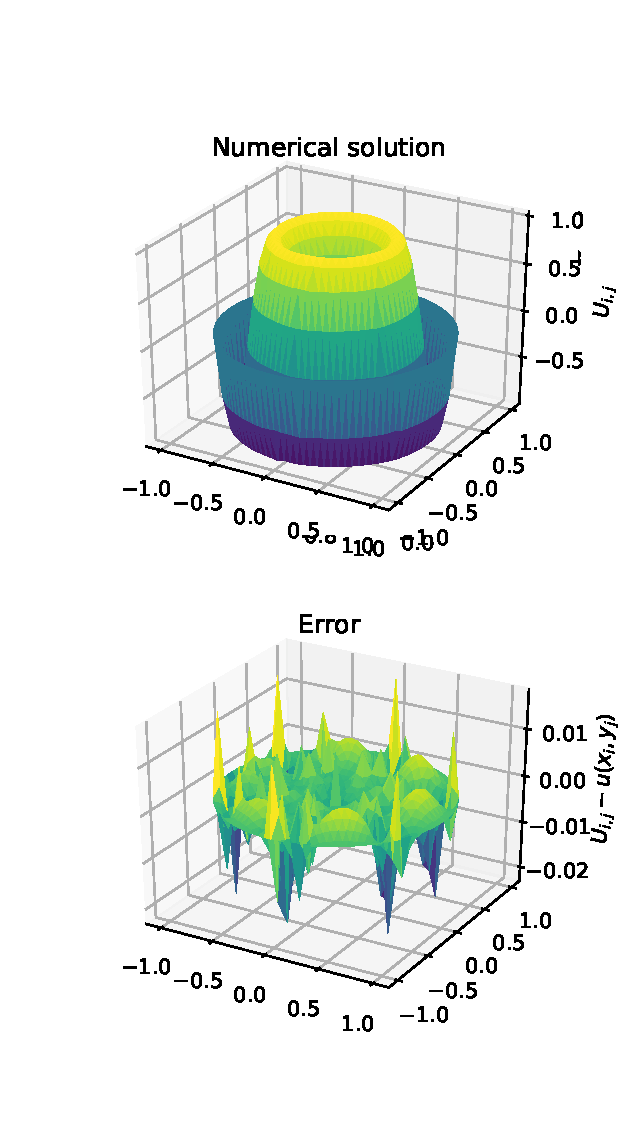
\includegraphics[scale=0.7]{solution_error.pdf}
    \caption{The poission problem solved on a disc mesh with $N = 1024$ nodes.
    The top plot displays the numerical solution from the Galerkin projection,
    while the bottom figure displays the error in the nodal points.}
    \label{solution-error}
\end{figure}

\begin{figure}[tbp]
    \centering
        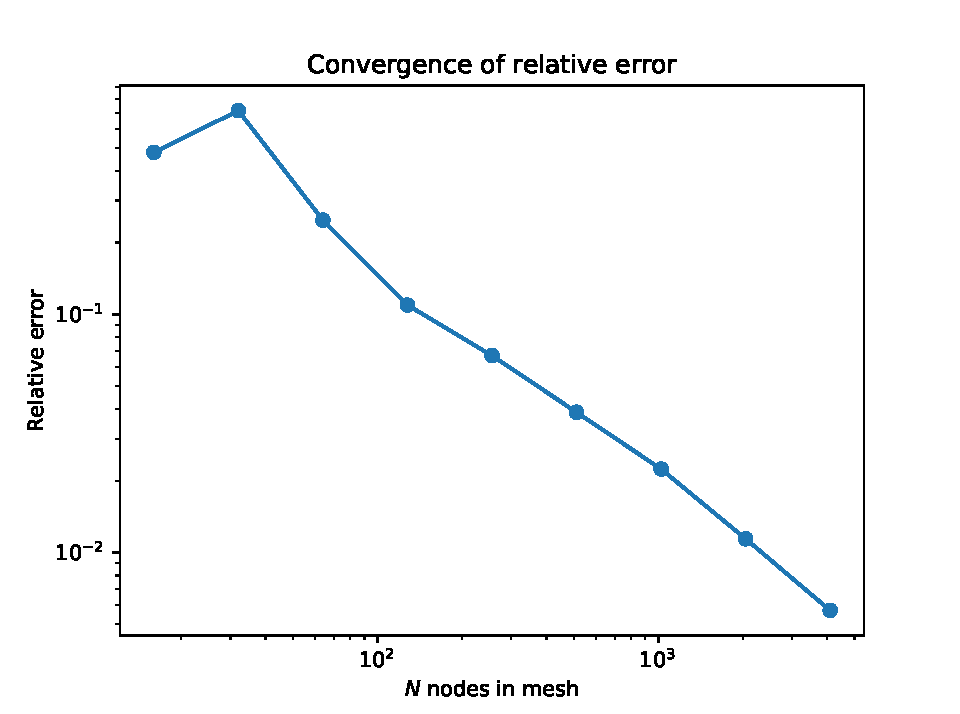
\includegraphics[scale=0.5]{convergence.pdf}
    \caption{Relative error when solving for multiple mesh discs with the number of nodes given by $N_n = \{ 2^n\}_{n=4}^{12}$
    where $N_{min} = 16$ and $N_{max} = 4096$.}
    \label{convergence}
\end{figure}

%%%%%%%%%%%%%%%%%%%%%%%%%%%%%%%%%%%%%%%%%%%%%%%%%%%%%%%%%%%%

\section{Diskusjon}
Lorem ipsum dolor sit amet, consectetur adipisicing elit, sed do eiusmod tempor incididunt ut labore et dolore magna aliqua. Ut enim ad minim veniam, quis nostrud exercitation ullamco laboris nisi ut aliquip ex ea commodo consequat. Duis aute irure dolor in reprehenderit in voluptate velit esse cillum dolore eu fugiat nulla pariatur. Excepteur sint occaecat cupidatat non proident, sunt in culpa qui officia deserunt mollit anim id est laborum.


%%%%%%%%%%%%%%%%%%%%%%%%%%%%%%%%%%%%%%%%%%%%%%%%%%%%%%%%%%%%%%%%%%%%%%%%%
\section{Konklusjon}
Lorem ipsum dolor \cite{dirac} sit amet, consectetur adipisicing elit, sed do eiusmod tempor incididunt ut labore et dolore magna aliqua. Ut enim ad minim veniam, quis nostrud exercitation ullamco laboris nisi ut aliquip ex ea commodo consequat. Duis aute irure dolor in reprehenderit in voluptate velit esse cillum dolore eu fugiat nulla pariatur. Excepteur sint occaecat cupidatat non proident, sunt in culpa qui officia deserunt mollit anim id est laborum.
	

\bibliography{ref}

\end{document}


